\documentclass{minimal}
\usepackage{tikz}

%\usetikzlibrary{shapes, }

\begin{document}

	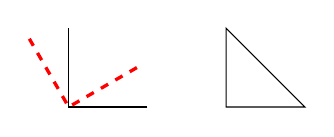
\begin{tikzpicture}
		\draw (1,0) -- (0,0) -- (0,1);
		\draw[red, dashed, very thick, rotate=30] (1,0) -- (0,0) -- (0,1);
		\draw (3,0) -- +(-1,0) -- +(-1,1) -- cycle;
	\end{tikzpicture}
	
	\vfill
	
	
\begin{tikzpicture}
		\draw (0,0) |- (1,1); % Pfad um die Ecke
		\draw [green, thick, fill=gray] (3,0) rectangle (5,1);
	\end{tikzpicture}
	
	\vfill
		
	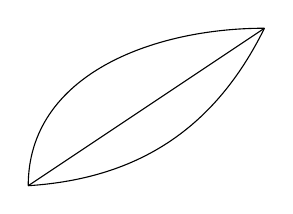
\begin{tikzpicture}
		\draw (0,0) to (3,2);
		\draw (0,0) to[out=90,in=180] (3,2);
		\draw (0,0) to[bend right] (3,2);
	\end{tikzpicture}
	
	\vfill
	
	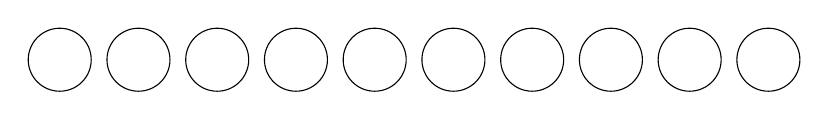
\begin{tikzpicture}
		\foreach \x in {0,...,9} \draw (\x,0) circle [radius=0.4];
	\end{tikzpicture}
	
	\vfill
	
	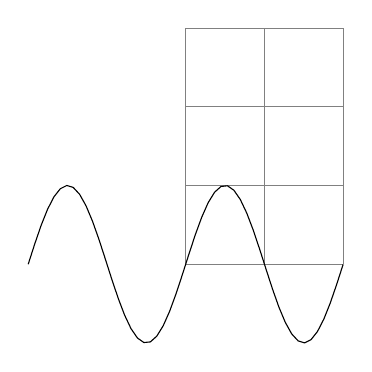
\begin{tikzpicture}
		\draw[help lines] (0,0) grid (2,3);
		\draw [domain=-2:2, samples=50] plot (\x, {sin(pi*\x r});
	\end{tikzpicture}
	
	\vfill
	
	\begin{tikzpicture}
		\draw (-1,0) to[bend left] (1,0);
		\draw (-1.2,.1) to[bend right] (1.2,.1);
		\draw (0,0) circle [x radius=100pt, y radius=50pt];
	\end{tikzpicture}

\end{document}
